\refstepcounter{section}
\section*{Lecture 2: Stability of Thermodynamic Systems}
\addcontentsline{toc}{section}{Lecture 2: Stability of Thermodynamic Systems}
We will discuss about the conditions under which the system in consideration is stable. This will in turn help us to understand \textit{phase transitions} which are consequences of instability! \\[0.2cm]

\begin{figure}[H]
    \centering
    

% Pattern Info
 
\tikzset{
pattern size/.store in=\mcSize, 
pattern size = 5pt,
pattern thickness/.store in=\mcThickness, 
pattern thickness = 0.3pt,
pattern radius/.store in=\mcRadius, 
pattern radius = 1pt}
\makeatletter
\pgfutil@ifundefined{pgf@pattern@name@_mfnjd2s2u}{
\pgfdeclarepatternformonly[\mcThickness,\mcSize]{_mfnjd2s2u}
{\pgfqpoint{0pt}{0pt}}
{\pgfpoint{\mcSize+\mcThickness}{\mcSize+\mcThickness}}
{\pgfpoint{\mcSize}{\mcSize}}
{
\pgfsetcolor{\tikz@pattern@color}
\pgfsetlinewidth{\mcThickness}
\pgfpathmoveto{\pgfqpoint{0pt}{0pt}}
\pgfpathlineto{\pgfpoint{\mcSize+\mcThickness}{\mcSize+\mcThickness}}
\pgfusepath{stroke}
}}
\makeatother
\tikzset{every picture/.style={line width=0.75pt}} %set default line width to 0.75pt        

\begin{tikzpicture}[x=0.75pt,y=0.75pt,yscale=-1,xscale=1]
%uncomment if require: \path (0,300); %set diagram left start at 0, and has height of 300

%Shape: Rectangle [id:dp7541659551963663] 
\draw  [fill={rgb, 255:red, 255; green, 255; blue, 255 }  ,fill opacity=1 ][line width=2.25]  (121.38,81) -- (440.06,81) -- (440.06,181.65) -- (121.38,181.65) -- cycle ;
%Shape: Rectangle [id:dp8756923650027149] 
\draw  [pattern=_mfnjd2s2u,pattern size=6pt,pattern thickness=0.75pt,pattern radius=0pt, pattern color={rgb, 255:red, 0; green, 0; blue, 0}][line width=1.5]  (275.75,80.82) -- (285.68,80.82) -- (285.68,181.82) -- (275.75,181.82) -- cycle ;
%Straight Lines [id:da7172550429347281] 
\draw    (321.68,126.65) -- (241.68,126.65) ;
\draw [shift={(239.68,126.65)}, rotate = 360] [color={rgb, 255:red, 0; green, 0; blue, 0 }  ][line width=0.75]    (10.93,-3.29) .. controls (6.95,-1.4) and (3.31,-0.3) .. (0,0) .. controls (3.31,0.3) and (6.95,1.4) .. (10.93,3.29)   ;
%Straight Lines [id:da9943390943743863] 
\draw    (171.68,106.65) -- (170.72,155.65) ;
\draw [shift={(170.68,157.65)}, rotate = 271.12] [color={rgb, 255:red, 0; green, 0; blue, 0 }  ][line width=0.75]    (10.93,-3.29) .. controls (6.95,-1.4) and (3.31,-0.3) .. (0,0) .. controls (3.31,0.3) and (6.95,1.4) .. (10.93,3.29)   ;
%Straight Lines [id:da17799970787124486] 
\draw    (393.68,107.65) -- (392.72,156.65) ;
\draw [shift={(392.68,158.65)}, rotate = 271.12] [color={rgb, 255:red, 0; green, 0; blue, 0 }  ][line width=0.75]    (10.93,-3.29) .. controls (6.95,-1.4) and (3.31,-0.3) .. (0,0) .. controls (3.31,0.3) and (6.95,1.4) .. (10.93,3.29)   ;

% Text Node
\draw (129,85.4) node [anchor=north west][inner sep=0.75pt]    {$S( U,V,N)$};
% Text Node
\draw (357,85.4) node [anchor=north west][inner sep=0.75pt]    {$S( U,V,N)$};
% Text Node
\draw (123,161.4) node [anchor=north west][inner sep=0.75pt]    {$S( U+\Delta U,V,N)$};
% Text Node
\draw (319,162.4) node [anchor=north west][inner sep=0.75pt]    {$S( U-\Delta U,V,N)$};
% Text Node
\draw (289,108.4) node [anchor=north west][inner sep=0.75pt]    {$\Delta U$};


\end{tikzpicture}

\end{figure}
\noindent
Consider two identical subsystems, with entropies $S(U,V,N)$, separated by an adiabatic wall. Suppose we remove an amount of energy $\Delta U$ from the first subsystem and transfer it to the second, the total energy changes from $2S(U,V,N)$ to $S(U+\Delta U)+S(U-\Delta U,V,N)$. Suppose that the entropy of the system looked something like in the diagram below. 
\begin{figure}[H]
    \centering

\tikzset{every picture/.style={line width=0.75pt}} %set default line width to 0.75pt        

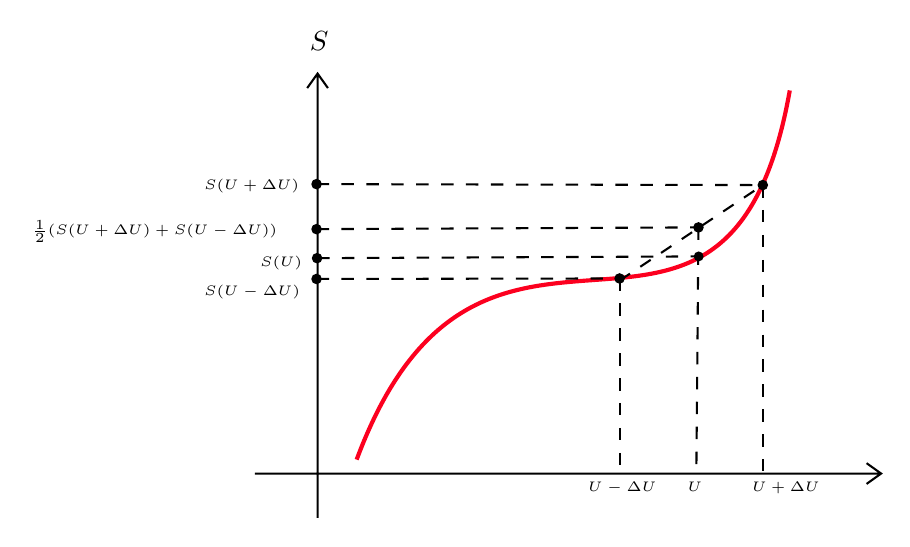
\begin{tikzpicture}[x=0.75pt,y=0.75pt,yscale=-1,xscale=1]
%uncomment if require: \path (0,300); %set diagram left start at 0, and has height of 300

%Shape: Axis 2D [id:dp8371481886954371] 
\draw  (151,247.72) -- (452.68,247.72)(181.17,55) -- (181.17,269.13) (445.68,242.72) -- (452.68,247.72) -- (445.68,252.72) (176.17,62) -- (181.17,55) -- (186.17,62)  ;
%Curve Lines [id:da9915347598713424] 
\draw [color={rgb, 255:red, 252; green, 0; blue, 31 }  ,draw opacity=1 ][line width=1.5]    (200,241) .. controls (260.68,78.13) and (378.68,232.13) .. (408.68,63.13) ;
%Straight Lines [id:da5338080977523495] 
\draw  [dash pattern={on 4.5pt off 4.5pt}]  (326.68,153.73) -- (326.68,247.43) ;
\draw [shift={(326.68,153.73)}, rotate = 90] [color={rgb, 255:red, 0; green, 0; blue, 0 }  ][fill={rgb, 255:red, 0; green, 0; blue, 0 }  ][line width=0.75]      (0, 0) circle [x radius= 2.01, y radius= 2.01]   ;
%Straight Lines [id:da5315894348525821] 
\draw  [dash pattern={on 4.5pt off 4.5pt}]  (364.68,129.13) -- (363.68,245.95) ;
\draw [shift={(364.68,129.13)}, rotate = 90.49] [color={rgb, 255:red, 0; green, 0; blue, 0 }  ][fill={rgb, 255:red, 0; green, 0; blue, 0 }  ][line width=0.75]      (0, 0) circle [x radius= 2.01, y radius= 2.01]   ;
%Straight Lines [id:da8144040544764883] 
\draw  [dash pattern={on 4.5pt off 4.5pt}]  (395.68,108.73) -- (395.68,247.57) ;
\draw [shift={(395.68,108.73)}, rotate = 90] [color={rgb, 255:red, 0; green, 0; blue, 0 }  ][fill={rgb, 255:red, 0; green, 0; blue, 0 }  ][line width=0.75]      (0, 0) circle [x radius= 2.01, y radius= 2.01]   ;
%Straight Lines [id:da6789218420069354] 
\draw  [dash pattern={on 4.5pt off 4.5pt}]  (326.68,154.73) -- (395.68,108.73) ;
%Shape: Circle [id:dp49363498746891266] 
\draw  [fill={rgb, 255:red, 0; green, 0; blue, 0 }  ,fill opacity=1 ] (362.93,143.11) .. controls (362.93,142.09) and (363.76,141.26) .. (364.78,141.26) .. controls (365.8,141.26) and (366.63,142.09) .. (366.63,143.11) .. controls (366.63,144.14) and (365.8,144.97) .. (364.78,144.97) .. controls (363.76,144.97) and (362.93,144.14) .. (362.93,143.11) -- cycle ;
%Straight Lines [id:da07316386568730371] 
\draw  [dash pattern={on 4.5pt off 4.5pt}]  (180.68,153.97) -- (326.68,153.73) ;
\draw [shift={(180.68,153.97)}, rotate = 359.91] [color={rgb, 255:red, 0; green, 0; blue, 0 }  ][fill={rgb, 255:red, 0; green, 0; blue, 0 }  ][line width=0.75]      (0, 0) circle [x radius= 2.01, y radius= 2.01]   ;
%Straight Lines [id:da8730317034140778] 
\draw  [dash pattern={on 4.5pt off 4.5pt}]  (180.68,129.97) -- (363.68,129.13) ;
\draw [shift={(180.68,129.97)}, rotate = 359.74] [color={rgb, 255:red, 0; green, 0; blue, 0 }  ][fill={rgb, 255:red, 0; green, 0; blue, 0 }  ][line width=0.75]      (0, 0) circle [x radius= 2.01, y radius= 2.01]   ;
%Straight Lines [id:da3224382986728025] 
\draw  [dash pattern={on 4.5pt off 4.5pt}]  (180.68,108.28) -- (395.68,108.73) ;
\draw [shift={(180.68,108.28)}, rotate = 0.12] [color={rgb, 255:red, 0; green, 0; blue, 0 }  ][fill={rgb, 255:red, 0; green, 0; blue, 0 }  ][line width=0.75]      (0, 0) circle [x radius= 2.01, y radius= 2.01]   ;
%Straight Lines [id:da003959848940690458] 
\draw  [dash pattern={on 4.5pt off 4.5pt}]  (180.93,143.95) -- (363.93,143.11) ;
\draw [shift={(180.93,143.95)}, rotate = 359.74] [color={rgb, 255:red, 0; green, 0; blue, 0 }  ][fill={rgb, 255:red, 0; green, 0; blue, 0 }  ][line width=0.75]      (0, 0) circle [x radius= 2.01, y radius= 2.01]   ;

% Text Node
\draw (176,33.4) node [anchor=north west][inner sep=0.75pt]    {$S$};
% Text Node
\draw (358,250.4) node [anchor=north west][inner sep=0.75pt]  [font=\tiny]  {$U$};
% Text Node
\draw (389,250.4) node [anchor=north west][inner sep=0.75pt]  [font=\tiny]  {$U+\Delta U$};
% Text Node
\draw (310,250.4) node [anchor=north west][inner sep=0.75pt]  [font=\tiny]  {$U-\Delta U$};
% Text Node
\draw (125,104.4) node [anchor=north west][inner sep=0.75pt]  [font=\tiny]  {$S(U+\Delta U)$};
% Text Node
\draw (125,155.4) node [anchor=north west][inner sep=0.75pt]  [font=\tiny]  {$S(U-\Delta U)$};
% Text Node
\draw (42,124.4) node [anchor=north west][inner sep=0.75pt]  [font=\tiny]  {$\frac{1}{2}\qty( S( U+\Delta U) +S( U-\Delta U))$};
% Text Node
\draw (152,141.4) node [anchor=north west][inner sep=0.75pt]  [font=\tiny]  {$S(U)$};


\end{tikzpicture}

\end{figure}
\noindent
Then, the resultant entropy after this transfer would be greater than the initial entropy. This would lead to inhomogenities in the system. Within one subsystem, there would be an uneven re-distribution of energy within different regions. This loss of homogenity indicated a \textit{phase separation}!\\[0.2cm]
Thus the stability condition is the \textit{concavity of entropy}, that is, 
\begin{equation}\label{eqn:global}
    S(U-\Delta U, V,N)+S(U+\Delta U, V,N)\leq 2S(U)
\end{equation}
Taylor expansion of the left hand side leads to the condition (under the limit $\Delta U \to 0$)
\begin{equation}\label{eqn:local}
    \boxed{\qty(\pdv[2]{S}{U})_{V,N}\leq 0}
\end{equation}
This implies that the curvature of the entropy should be downwards! It might happen that we obtain a `locally convex' entropy curve from some calculation or from experimental data, which does not obey concavity.

\begin{figure}[H]
    \centering 
    

\tikzset{every picture/.style={line width=0.75pt}} %set default line width to 0.75pt        

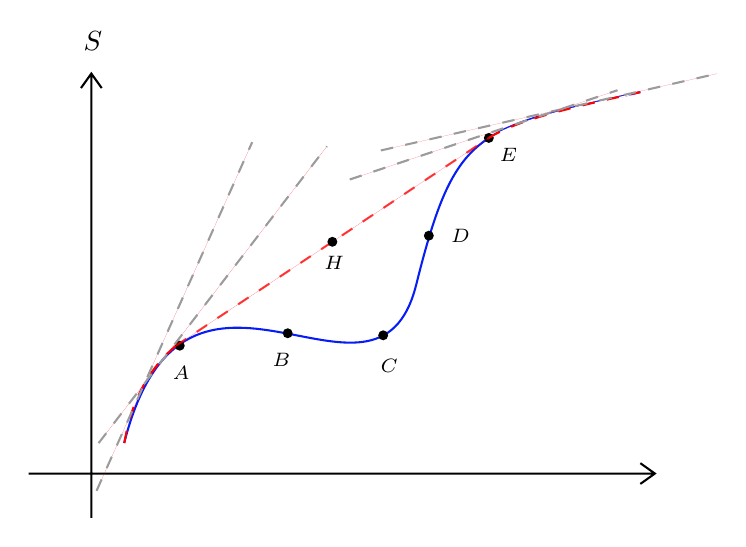
\begin{tikzpicture}[x=0.75pt,y=0.75pt,yscale=-1,xscale=1]
%uncomment if require: \path (0,300); %set diagram left start at 0, and has height of 300

%Shape: Axis 2D [id:dp18223659738412512] 
\draw  (162,241.72) -- (463.68,241.72)(192.17,49) -- (192.17,263.13) (456.68,236.72) -- (463.68,241.72) -- (456.68,246.72) (187.17,56) -- (192.17,49) -- (197.17,56)  ;
%Curve Lines [id:da3459358101363742] 
\draw [color={rgb, 255:red, 7; green, 29; blue, 245 }  ,draw opacity=1 ][line width=0.75]    (208,227) .. controls (237.68,109.95) and (329.68,226.78) .. (348.68,150.78) .. controls (367.68,74.78) and (377.68,75.78) .. (456.68,57.95) ;
%Shape: Circle [id:dp8318209744444434] 
\draw  [fill={rgb, 255:red, 0; green, 0; blue, 0 }  ,fill opacity=1 ] (232.93,180.11) .. controls (232.93,179.09) and (233.76,178.26) .. (234.78,178.26) .. controls (235.8,178.26) and (236.63,179.09) .. (236.63,180.11) .. controls (236.63,181.14) and (235.8,181.97) .. (234.78,181.97) .. controls (233.76,181.97) and (232.93,181.14) .. (232.93,180.11) -- cycle ;
%Shape: Circle [id:dp6035913035404311] 
\draw  [fill={rgb, 255:red, 0; green, 0; blue, 0 }  ,fill opacity=1 ] (381.83,80.02) .. controls (381.83,78.99) and (382.66,78.16) .. (383.68,78.16) .. controls (384.71,78.16) and (385.54,78.99) .. (385.54,80.02) .. controls (385.54,81.04) and (384.71,81.87) .. (383.68,81.87) .. controls (382.66,81.87) and (381.83,81.04) .. (381.83,80.02) -- cycle ;
%Straight Lines [id:da30749443542169463] 
\draw [color={rgb, 255:red, 255; green, 0; blue, 0 }  ,draw opacity=0.76 ][fill={rgb, 255:red, 255; green, 0; blue, 31 }  ,fill opacity=1 ] [dash pattern={on 4.5pt off 4.5pt}]  (232.93,180.11) -- (383.68,80.02) ;
%Shape: Circle [id:dp5221148012759685] 
\draw  [fill={rgb, 255:red, 0; green, 0; blue, 0 }  ,fill opacity=1 ] (284.93,174.11) .. controls (284.93,173.09) and (285.76,172.26) .. (286.78,172.26) .. controls (287.8,172.26) and (288.63,173.09) .. (288.63,174.11) .. controls (288.63,175.14) and (287.8,175.97) .. (286.78,175.97) .. controls (285.76,175.97) and (284.93,175.14) .. (284.93,174.11) -- cycle ;
%Shape: Circle [id:dp16192304439779115] 
\draw  [fill={rgb, 255:red, 0; green, 0; blue, 0 }  ,fill opacity=1 ] (330.93,175.11) .. controls (330.93,174.09) and (331.76,173.26) .. (332.78,173.26) .. controls (333.8,173.26) and (334.63,174.09) .. (334.63,175.11) .. controls (334.63,176.14) and (333.8,176.97) .. (332.78,176.97) .. controls (331.76,176.97) and (330.93,176.14) .. (330.93,175.11) -- cycle ;
%Shape: Circle [id:dp6212521734834506] 
\draw  [fill={rgb, 255:red, 0; green, 0; blue, 0 }  ,fill opacity=1 ] (352.93,127.11) .. controls (352.93,126.09) and (353.76,125.26) .. (354.78,125.26) .. controls (355.8,125.26) and (356.63,126.09) .. (356.63,127.11) .. controls (356.63,128.14) and (355.8,128.97) .. (354.78,128.97) .. controls (353.76,128.97) and (352.93,128.14) .. (352.93,127.11) -- cycle ;
%Curve Lines [id:da9027146588706242] 
\draw [color={rgb, 255:red, 255; green, 0; blue, 0 }  ,draw opacity=1 ][fill={rgb, 255:red, 255; green, 255; blue, 255 }  ,fill opacity=1 ][line width=0.75]  [dash pattern={on 4.5pt off 4.5pt}]  (383.68,80.02) .. controls (397.68,71.1) and (424.68,65.1) .. (456.68,57.95) ;
%Curve Lines [id:da6266906447332434] 
\draw [color={rgb, 255:red, 255; green, 0; blue, 0 }  ,draw opacity=1 ][line width=0.75]  [dash pattern={on 4.5pt off 4.5pt}]  (208,227) .. controls (208.68,225.88) and (210.68,198.88) .. (232.93,180.11) ;
%Shape: Circle [id:dp2802498605440815] 
\draw  [fill={rgb, 255:red, 0; green, 0; blue, 0 }  ,fill opacity=1 ] (306.45,130.06) .. controls (306.45,129.04) and (307.28,128.21) .. (308.3,128.21) .. controls (309.33,128.21) and (310.16,129.04) .. (310.16,130.06) .. controls (310.16,131.09) and (309.33,131.92) .. (308.3,131.92) .. controls (307.28,131.92) and (306.45,131.09) .. (306.45,130.06) -- cycle ;
%Straight Lines [id:da7015012094242393] 
\draw [color={rgb, 255:red, 155; green, 155; blue, 155 }  ,draw opacity=1 ][fill={rgb, 255:red, 255; green, 0; blue, 31 }  ,fill opacity=1 ] [dash pattern={on 4.5pt off 4.5pt}]  (194.68,250.05) -- (269.68,82.05) ;
%Straight Lines [id:da22294183965749914] 
\draw [color={rgb, 255:red, 155; green, 155; blue, 155 }  ,draw opacity=1 ][fill={rgb, 255:red, 255; green, 0; blue, 31 }  ,fill opacity=1 ] [dash pattern={on 4.5pt off 4.5pt}]  (195.68,227.05) -- (305.68,84.05) ;
%Straight Lines [id:da7838813020303588] 
\draw [color={rgb, 255:red, 155; green, 155; blue, 155 }  ,draw opacity=1 ][fill={rgb, 255:red, 255; green, 0; blue, 31 }  ,fill opacity=1 ] [dash pattern={on 4.5pt off 4.5pt}]  (331.68,86.05) -- (493.68,49.05) ;
%Straight Lines [id:da7411384547782376] 
\draw [color={rgb, 255:red, 155; green, 155; blue, 155 }  ,draw opacity=1 ][fill={rgb, 255:red, 255; green, 0; blue, 31 }  ,fill opacity=1 ] [dash pattern={on 4.5pt off 4.5pt}]  (316.68,100.05) -- (445.68,57.05) ;

% Text Node
\draw (187,27.4) node [anchor=north west][inner sep=0.75pt]    {$S$};
% Text Node
\draw (230,188.4) node [anchor=north west][inner sep=0.75pt]  [font=\scriptsize]  {$A$};
% Text Node
\draw (278,182.4) node [anchor=north west][inner sep=0.75pt]  [font=\scriptsize]  {$B$};
% Text Node
\draw (330,185.4) node [anchor=north west][inner sep=0.75pt]  [font=\scriptsize]  {$C$};
% Text Node
\draw (364,122.4) node [anchor=north west][inner sep=0.75pt]  [font=\scriptsize]  {$D$};
% Text Node
\draw (387.54,83.42) node [anchor=north west][inner sep=0.75pt]  [font=\scriptsize]  {$E$};
% Text Node
\draw (303,135.4) node [anchor=north west][inner sep=0.75pt]  [font=\scriptsize]  {$H$};


\end{tikzpicture}

\end{figure}
\noindent
This \textit{convex intruder} cannot describe the equilibrium state and we have to obtain the \textit{stable thermodynamic fundamental equation} from this curve. To do that, we construct all the \textit{superior tangents}, that is, tangents which are above this curve. Now, within the family of tangents, there will be one line which will touch the curve at two places.\\[0.2cm] In the diagram, tangent at any point after A (but before E) will cross the curve. Now, the tangent at A will touch the curve at E. If it had not touched, it would have either intersected the curve or gone above E (If it has intersected the curve, then the tangent at A should not have been considered at all since we are considering only superior tangents. If it had gone over E, this means that there must be some points after A, where this touching will occur. In any case, what we want to say is that, there will be a `common tangent' at points A and E). \\[0.2cm]
Now, take the envelope of this family of tangents and this will be the fundamental thermodynamic equation that describes the equilibirum states.\\[0.2cm]
Any point on the straight line denotes a phase-separated state, where part of the system is in state A and another part is in E. This happens because of the convex curve of entropy, which creates an inhomogenity.  \\[0.2cm]
Note that in the region AB and DE, entropy is still concave, hence these are called \textit{metastable} or locally stable states. These states satisfy Eq.\eqref{eqn:local} but does not satisfy Eq.\eqref{eqn:global} while the region BCD satisfy neither condition.
\subsection{Stability Relations for Potentials}
We will now discuss what are the consequence of stability on the thermodynamic potentials, $F$ and $G$. We will use the fact that for a mechanically stable system, the \textit{specific heat} and the \textit{thermal compressibility} must be positive for all temperatures. It can be motivated since compressibility and specific heat are related to number and energy fluctuations, $\sigma\tund{N}$ and $\sigma\tund{E}$ respectively, both of which are positive.\\[0.2cm]
From appendix \ref{appendix:legendre}, we see that $S = -\qty(\pdv{F}{T})_{V,N}$ from which we get:
$$\qty(\pdv[2]{F}{T})_{V,N} = - \qty(\pdv{S}{T})_{V,N} = -\frac{1}{T}C_v \leq 0$$
Similarly, we can use $S = -\qty(\pdv{G}{T})_{P,N}$ from which we get:
$$\qty(\pdv[2]{G}{T})_{P,N} = - \qty(\pdv{S}{T})_{P,N} = -\frac{1}{T}C_p \leq 0$$
From this, we infer that $G(T,P,N)$ and $F(T,V,N)$ are concave functions of temperature. Apart from temperature, since $F$ depends on $V$ and $G$ depends on P, let us check for pressure and volume too. We note that $V = -\qty(\pdv{G}{P})_{T,N}$ and $P = -\qty(\pdv{F}{V})_{T,N}$
\begin{align}\label{eqn:potential}
    \begin{split}
        \qty(\pdv[2]{G}{P})_{T,N} &= - \qty(\pdv{V}{P})_{T,N} = -VK\tund{T} \leq 0\\
    \qty(\pdv[2]{F}{V})_{T,N} &= - \qty(\pdv{P}{V})_{P,N} = \frac{1}{VK\tund{T}} \geq 0
    \end{split}
\end{align}
where we have appropriately used the definitions of thermal compressibility and heat capacity. Using this, we find that $G$ is a concave function of pressure and $F$ is a convex function of volume. From the above expressions in Eq \ref{eqn:potential}, we can also write 
$$ \qty(\pdv[2]{G}{P})_{T,N} = -\qty{\qty(\pdv[2]{F}{V})_{T,N}}^{-1}$$
\subsection{Stability Analysis of Van der waal's solutions}
Recall the Van der Waal's equation from Eq \eqref{eqn:vander},
$$\qty(P+\frac{aN^2}{V^2})\qty(V-Nb) = N\kb T$$
At high temperature, the $P$ vs. $V$ curves at constant temperature (\textit{isotherm}) follows the usual ideal-gas curve. However, there exists a critical temperature $T\tund{c}$ (which can be found out from the equation), such that, for $T<T\tund{c}$, there always exist a region, where the slope $\pdv{P}{V}$ is positive. Since $K\tund{T} = -\frac{1}{V}\qty(\pdv{V}{P})_{N,T}$, this implies a negative compressibility, which, as motivated before, is \textit{unphysical}.\\[0.2cm]
This leads to a breakdown of the theory and Maxwell subsequently proposed an \textit{ad hoc} remedy, similar in line to the construction of superior tangents that we noted earlier. 
\begin{figure}[H]
    \centering 
    

\tikzset{every picture/.style={line width=0.75pt}} %set default line width to 0.75pt        

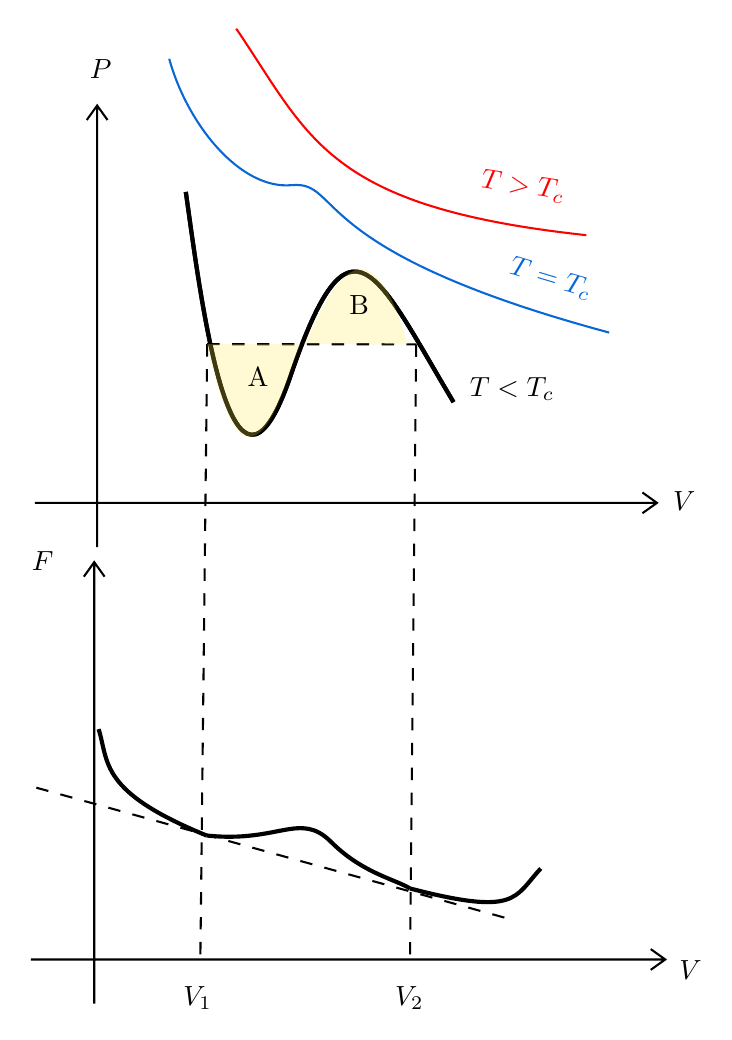
\begin{tikzpicture}[x=0.75pt,y=0.75pt,yscale=-1,xscale=1]
%uncomment if require: \path (0,527); %set diagram left start at 0, and has height of 527

%Shape: Axis 2D [id:dp970091110037609] 
\draw  (51,254.44) -- (350.68,254.44)(80.97,63) -- (80.97,275.72) (343.68,249.44) -- (350.68,254.44) -- (343.68,259.44) (75.97,70) -- (80.97,63) -- (85.97,70)  ;
%Shape: Axis 2D [id:dp5002897351550694] 
\draw  (49,474.44) -- (354.68,474.44)(79.57,283) -- (79.57,495.72) (347.68,469.44) -- (354.68,474.44) -- (347.68,479.44) (74.57,290) -- (79.57,283) -- (84.57,290)  ;
%Curve Lines [id:da45956577782421615] 
\draw [line width=1.5]    (123.68,104.65) .. controls (130.72,153.89) and (145.48,277.34) .. (174.31,192.83) .. controls (203.14,108.32) and (215.68,143.92) .. (252.68,205.92) ;
%Curve Lines [id:da823430407451243] 
\draw [line width=1.5]    (123.68,104.65) .. controls (130.72,153.89) and (145.48,277.34) .. (174.31,192.83) .. controls (203.14,108.32) and (215.68,143.92) .. (252.68,205.92) ;

%Straight Lines [id:da11792893756552392] 
\draw  [dash pattern={on 4.5pt off 4.5pt}]  (134,178) -- (234.68,178.05) ;
%Straight Lines [id:da15895122499938086] 
\draw  [dash pattern={on 4.5pt off 4.5pt}]  (134,178) -- (130.68,475.37) ;
%Straight Lines [id:da8118475157989993] 
\draw  [dash pattern={on 4.5pt off 4.5pt}]  (234.68,178.05) -- (231.68,476.37) ;
%Straight Lines [id:da09683450161007845] 
\draw  [dash pattern={on 4.5pt off 4.5pt}]  (51.68,391.67) -- (278.68,454.67) ;
%Curve Lines [id:da021972733689352486] 
\draw [line width=1.5]    (133.68,414.7) .. controls (168.68,418.45) and (178.68,402.8) .. (193.68,417.8) .. controls (208.68,432.8) and (224.68,435.8) .. (231.68,440.23) ;
%Curve Lines [id:da2284935025874082] 
\draw [line width=1.5]    (231.68,440.23) .. controls (283.68,453.62) and (281.68,444.62) .. (294.68,430.62) ;
%Curve Lines [id:da760370312377808] 
\draw [line width=1.5]    (133.68,414.7) .. controls (81.68,393.45) and (86.68,379.45) .. (81.68,363.45) ;
%Shape: Boxed Bezier Curve [id:dp5322575875876991] 
\draw [color={rgb, 255:red, 255; green, 0; blue, 0 }  ,draw opacity=1 ]   (148,26) .. controls (183.45,78.08) and (190.94,111.93) .. (316.68,125.47) ;
%Shape: Boxed Bezier Curve [id:dp7587016286783995] 
\draw [color={rgb, 255:red, 8; green, 103; blue, 215 }  ,draw opacity=1 ]   (115.68,40.47) .. controls (124.45,72.24) and (149.95,103.61) .. (174.66,101.37) .. controls (199.37,99.14) and (180.24,132.68) .. (327.68,172.4) ;
%Shape: Path Data [id:dp7034407204988964] 
\draw  [draw opacity=0][fill={rgb, 255:red, 255; green, 235; blue, 78 }  ,fill opacity=0.25 ][line width=0.75]  (173.01,193.83) .. controls (155.07,246.42) and (142.57,218.48) .. (134,178) -- (178.77,178) .. controls (176.92,182.72) and (175,187.99) .. (173.01,193.83) -- cycle ;
%Shape: Path Data [id:dp6192702070359754] 
\draw  [draw opacity=0][fill={rgb, 255:red, 255; green, 235; blue, 78 }  ,fill opacity=0.25 ][line width=0.75]  (187.2,165.13) .. controls (207.36,122.74) and (221.19,145.37) .. (230.61,178.1) -- (180.73,177.9) .. controls (182.81,174.09) and (184.96,169.84) .. (187.2,165.13) -- cycle ;

% Text Node
\draw (76,39.4) node [anchor=north west][inner sep=0.75pt]    {$P$};
% Text Node
\draw (357,247.4) node [anchor=north west][inner sep=0.75pt]    {$V$};
% Text Node
\draw (360,473.4) node [anchor=north west][inner sep=0.75pt]    {$V$};
% Text Node
\draw (48,276.4) node [anchor=north west][inner sep=0.75pt]    {$F$};
% Text Node
\draw (265.7,91.6) node [anchor=north west][inner sep=0.75pt]  [color={rgb, 255:red, 255; green, 0; blue, 0 }  ,opacity=1 ,rotate=-8.82]  {$T >T_{c}$};
% Text Node
\draw (280.7,133.44) node [anchor=north west][inner sep=0.75pt]  [color={rgb, 255:red, 8; green, 103; blue, 215 }  ,opacity=1 ,rotate=-16.74]  {$T=T_{c}$};
% Text Node
\draw (259,192.4) node [anchor=north west][inner sep=0.75pt]  [color={rgb, 255:red, 0; green, 0; blue, 0 }  ,opacity=1 ]  {$T<T_{c}$};
% Text Node
\draw (121,486.12) node [anchor=north west][inner sep=0.75pt]    {$V_{1}$};
% Text Node
\draw (223,486.1) node [anchor=north west][inner sep=0.75pt]    {$V_{2}$};
% Text Node
\draw (152,188) node [anchor=north west][inner sep=0.75pt]   [align=left] {A};
% Text Node
\draw (201,153) node [anchor=north west][inner sep=0.75pt]   [align=left] {B};


\end{tikzpicture}

\end{figure}
\noindent
Consider the diagram above. Here, for a subcritical temperature, we see a region between $V_1$ and $V_2$ where the slope is positive. This region corresponds to the \textit{concave intruder} (since free energy is a convex function of volume) in the free energy plot. Similarly as before, we replaced the concave part with a straight line denoting the commong tangent. This corresponds to joining the region between $V_1$ and $V_2$ in the P-V plot with a straight horizontal line. It can also be shown that the horizontal line is at just such a value of the pressure that the areas labelled A and B are equal and hence this construction is also called \textit{equal-area} construction. 
